%%%%
% Преамбула: подключение необходимых пакетов
% Редактируйте осторожно!
%

\documentclass[hyperref={unicode}]{beamer}

\usepackage[utf8x]{inputenc}
\usepackage[english, russian]{babel}
\usepackage{color, colortbl}
\usepackage{rotating} 
\usepackage{graphicx}
\usepackage{algorithmic}

\usetheme[nosecheader]{PetrSU-CS}


%%%%
% Преамбула: основные параметры презентации
% Отредактируйте в соответствии с комментариями
%

\title[%
	% Краткое название работы не используется в этой презентации!
		Сайт для переводов
]{%
		% Полное название работы отображается на титульной странице
		Создание веб-сервиса\\ 
		для коллективных переводов
}

% Подзаголовком опишите тип работы:
% - Курсовая работа
% - Выпускная квалификационная работа бакалавра
% - Дипломная работа
% - Магистерская диссертация
\subtitle{Промежуточный отчет о научно-исследовательской работе}

\author[%
		% Имя и фамилия автора работы отображаются на каждом слайде в нижнем колонтитуле
		Зименкова С., Смирнов Е.
]{%
		% Имя, отчество и фамилия автора работы отображаются на титульном слайде
		Зименкова С. Э., Смирнов Е. Р.
}

\date[%
		% Дата защиты
		25.12.2022
]{%
		% Руководитель
		Научный руководитель: Д. Б. Чистяков
}

\institute[%
		% Краткое название организации не используется в этой презентации
		ПетрГУ
]{%
		% Полное название организации и подразделения
		Петрозаводский государственный университет\\
		Кафедра Информатики и Математического Обеспечения
}


%%%%
%
% Начало содержимого слайдов
%

\begin{document}

% Титульный слайд
\begin{frame}
\maketitle
\end{frame}

% Пример слайда для обоснования актуальности работы
\begin{frame}
	% Заголовок слайда
	\frametitle{Требования к сервису}
	Для организации эффективной работы коллектива переводчиков инструмент должен иметь следующие фукнции:
 \begin{itemize}
		\item загрузка текста и определение участников его перевода;
		\item разбиение исходного текста на главы и фрагменты;
		\item распределение задач и ролей между участниками перевода;
		\item сихнронизация материалов и прогресса между участниками перевода;
		\item выбор и утверждение наилучшего варианта перевода;
		\item выгрузка итогового текста.
	\end{itemize}
	
	Эти функции удобно реализовать с помощью веб-сервиса, поэтому инструмент будет реализован в виде сайта.
	
	%\begin{center}
	%	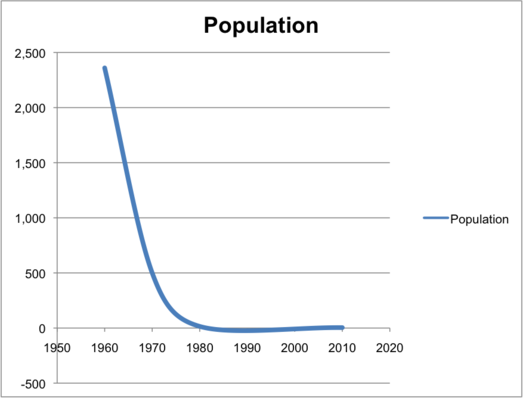
\includegraphics[width=0.4\textwidth]{images/pop.png}
	%\end{center}
	
	
\end{frame}

% Пример слайда с формулировкой целей и задач
\begin{frame}
	% Заголовок слайда
	\frametitle{Цель и задачи}
	\begin{block}{Цель работы}
		%Разработать основу веб-сервиса для коллективных переводов.
		Разработать веб-сервис для коллективных переводов.
	\end{block}
	\begin{block}{Задачи}
	\begin{itemize}
		\item разработать модель структуры внутреннего представления объектов веб-сервиса;
		\item создать наброски дизайна пользовательского интерфейса;
		\item разработать компоненты веб-сервиса:
		\begin{itemize}
			\item веб-API;
			\item базы данных;
			\item шаблоны веб-страниц.
		\end{itemize}
	\end{itemize}
	\end{block}
\end{frame}

% % Пример слайда содержащего код
% \begin{frame}[fragile]
% 	% Заголовок слайда
% 	\frametitle{Алгоритм расчета поголовья бобров}
% 	\framesubtitle{(оформляем фрагмент исходного кода или псевдокода)}
	
% 	\begin{verbatim}
% 		цикл для всех водоемов
% 			цикл для всех хаток
% 				если хатка не брошена, то
% 					sum += количество бобров в текущей хатке
% 				конец условия
% 			конец цикла по хаткам
% 		конец цикла по водоемам
% 	\end{verbatim}
	
% \end{frame}

% % Пример заключительного слайда
% \begin{frame}
% 	\frametitle{Заключение}
	
% 	Полученные результаты
	
% 	\begin{itemize}
% 		\item Изучено ...
% 		\item Построено ...
% 		\item Спроектировано ...
% 		\item Реализовано ...
% 		\item Опубликовано ...
% 		\item Внедрено ... 
% 	\end{itemize}
	
% \end{frame}

% \begin{frame}
% 	\frametitle{}
	
% {\Large\mbox{}\hfil Спасибо за внимание!}
	
% \end{frame}
\end{document}
